% file: reasoning_case.tex
\begin{ReasoningBox}[title=Question Understanding Error] % 可以通过 title 参数修改标题
    % --- 第一部分：问题描述与图片 ---
    % \begin{minipage}[t]{0.58\textwidth}
        \textbf{Question:} Based on the daily runoff water level time series data from 5 river sensors in East Germany, which adjacency matrix most accurately describes the causal relationship between them? In the matrix, columns represent 'cause' nodes, rows represent 'result' nodes, and '1' indicates the presence of causal effects.
    % \end{minipage}%
    % \hfill
    

    \vspace{0.5em}

    % --- 第二部分：选项 ---
    \textbf{Answer Choices:} 
    % --- Option A (Matrix 1: 3->2, 1->3, 4->3, 5->3) ---
    (A) \causalGraph{
        \draw[edge style] (3) -- (2);
        \draw[edge style] (1) -- (3);
        \draw[edge style] (4) -- (3);
        \draw[edge style] (5) -- (3);
    } \hfill
    % --- Option B (Matrix 2: 1->3, 4->3, 5->3, 3->4) ---
    (B) \causalGraph{
        \draw[edge style] (1) -- (3);
        \draw[edge style] (4) -- (3);
        \draw[edge style] (5) -- (3);
        \draw[edge style] (2) -- (4);
    } \hfill
    % --- Option C (Matrix 3: 3->1, 2->3, 3->4, 3->5) [CORRECT] ---
    (C) \causalGraph{
        \draw[edge style] (3) -- (1);
        \draw[edge style] (2) -- (3);
        \draw[edge style] (3) -- (4);
        \draw[edge style] (3) -- (5);
    } \hfill
    % --- Option D (Matrix 4: 3->2, 1->3, 2->3, 5->3) [MODEL ERROR] ---
    (D) \causalGraph{
        \draw[edge style] (3) -- (2);
        \draw[edge style] (1) -- (3);
        \draw[edge style] (3) -- (4);
        \draw[edge style] (5) -- (3);
    }
    \vspace{10pt}
    \\
    
    \noindent\textbf{Correct Answer:} \textcolor{correctgreen}{(A)} \\
    \textbf{Model Answer:} \textcolor{wrongred}{(D)}
    
    \vspace{0.3em}
    \begin{wrapfigure}{r}{0.6\textwidth}
        \centering
        % wrapfigure 通常顶部会有多余空白，使用负 vspace 向上提，让图片和第一行文字对齐
        \vspace{-45pt} 
        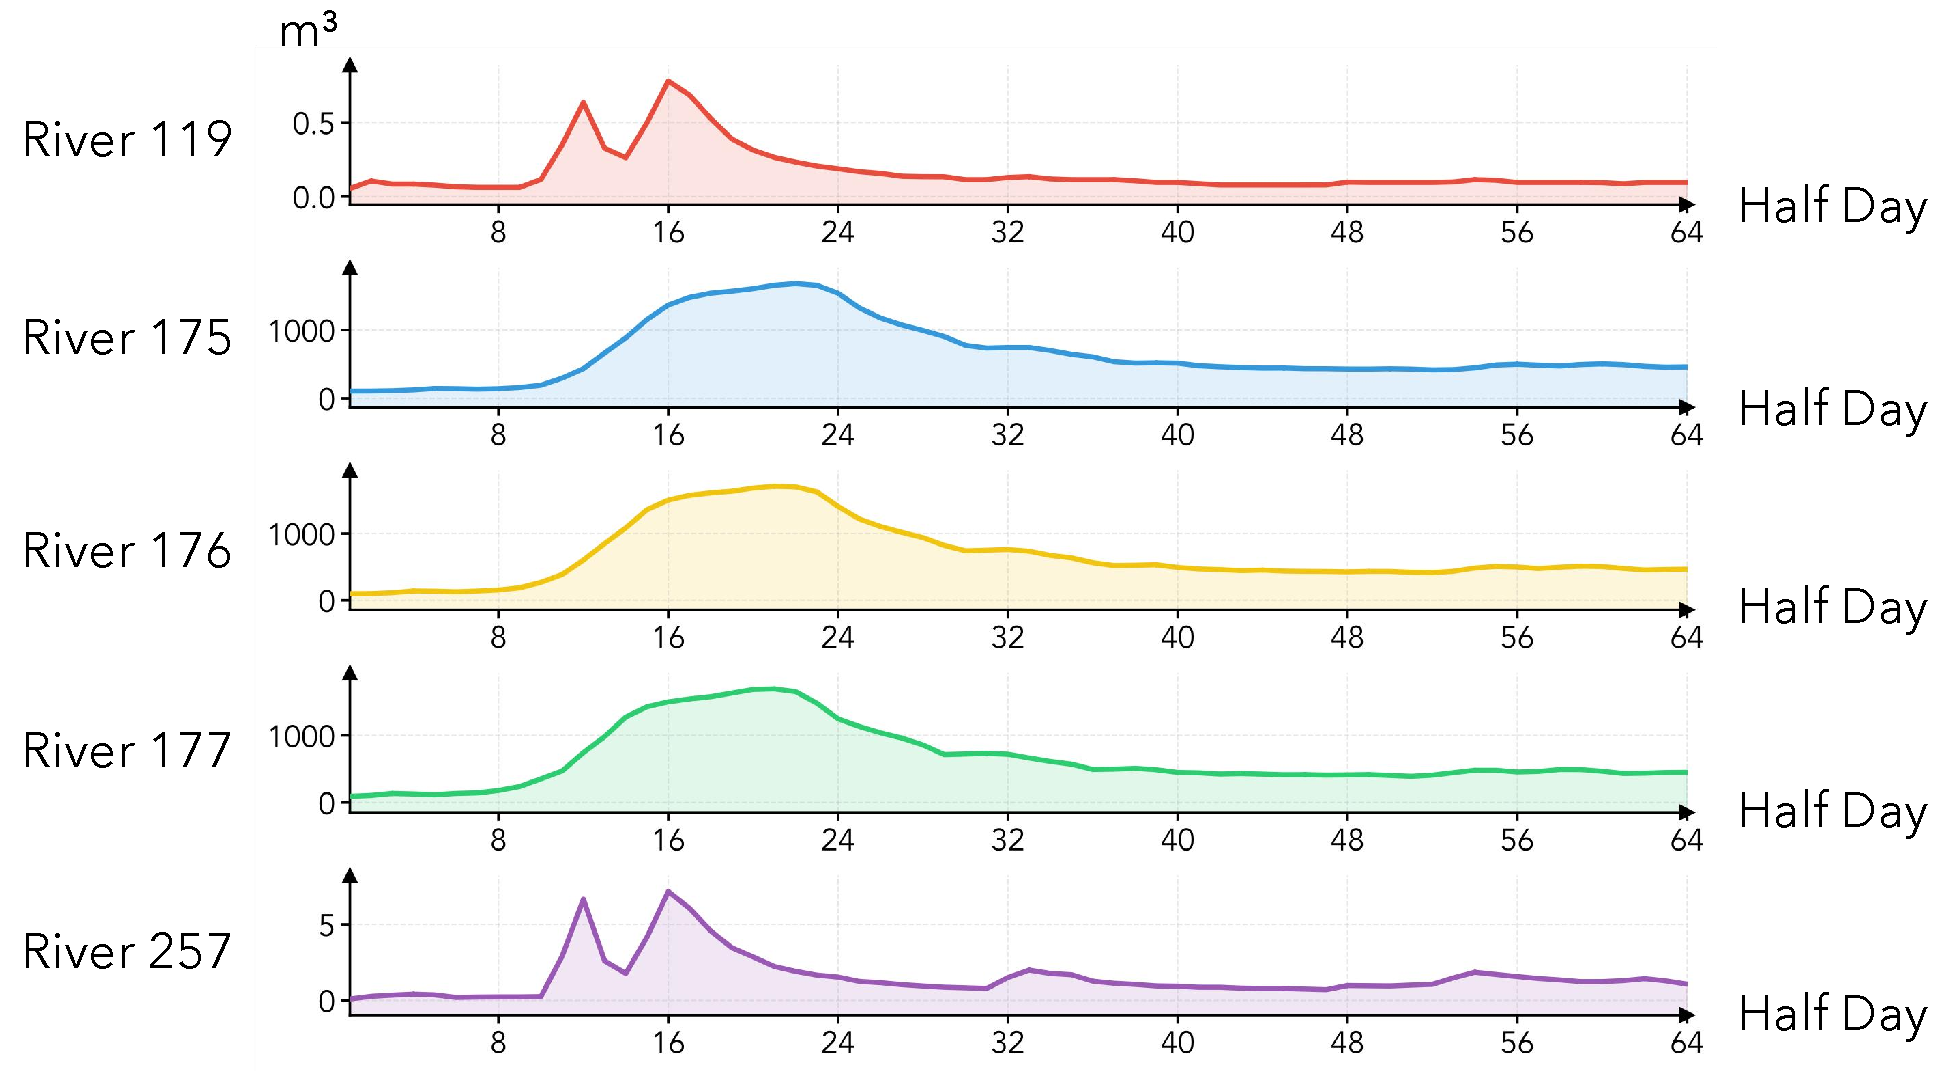
\includegraphics[width=0.95\linewidth]{blocks/case_study_figs/question_error.pdf}
        % 调整底部的留白
        \vspace{-10pt}
    \end{wrapfigure}
    % --- 第四部分：基本原理 (Rationale) ---
    \textbf{Prediction Rationale:} To determine the most accurate adjacency matrix, I first need to understand the relationships between the time series data of the rivers. The rivers with higher magnitudes in their time series (e.g., River 175, 176, 177) show large spikes, suggesting possible influence from upstream rivers. River 119 and 257 have lower and more consistent values, likely being affected by the larger rivers. Analyzing the options, the matrix that best reflects causal relationships from the larger rivers to the others is option D. It indicates that River 176 (second row) influences River 175, and River 175 influences others (first row), which aligns with the observed data patterns.\\
    
    \par            % 确保结束上一段
    % \vspace{0.8em}  % 调整上方留白
    \hrule          % 绘制横线
    \vspace{0.8em}  % 调整下方留白
    \textbf{Error Analysis:} \textit{The model misinterpreted the adjacency matrix orientation specified in the question. The prompt clearly states that columns represent 'cause' nodes and rows represent 'result' nodes. However, in its justification, the model said “the matrix indicates that River 176 (second row) influences River 175,” which treats rows as causes rather than results. This inversion leads to a fundamentally wrong reading of edges in option D (e.g., D[2,3]=1 actually means node 3 causes node 2, not that row 2 causes row 3). While the model also relied on a weak heuristic (magnitude/spikes imply causality), the decisive error is the matrix semantics misunderstanding, which directly corrupted the mapping from observed relationships to matrix entries and explains the selection of D over the ground truth A.}
\end{ReasoningBox}